\documentclass[12pt,a4paper]{article}

\usepackage[a4paper,margin=2.2cm]{geometry}
\usepackage[T2A]{fontenc}
\usepackage[utf8]{inputenc}
\usepackage[russian]{babel}
\usepackage{amsmath,amssymb,amsthm}
\usepackage{graphicx}
\usepackage{float}
\usepackage{booktabs}
\usepackage{hyperref}
\usepackage{enumitem}
\usepackage{setspace}
\usepackage{caption}

\setlength{\parindent}{1.25cm}
\setlength{\parskip}{0.25em}
\onehalfspacing

\newcommand{\imgplaceholder}[2]{%
\begin{figure}[H]
\centering
\fbox{%
  \begin{minipage}[c][0.22\textheight][c]{0.85\textwidth}
  \centering
  \textbf{Заглушка для изображения}\\[0.5em]
  #2
  \end{minipage}}
\caption{#1}
\end{figure}}

\begin{document}

\begin{titlepage}
\centering
{\large МОСКОВСКИЙ ФИЗИКО-ТЕХНИЧЕСКИЙ ИНСТИТУТ\\
(НАЦИОНАЛЬНЫЙ ИССЛЕДОВАТЕЛЬСКИЙ УНИВЕРСИТЕТ)\\
Кафедра общей физики\par}
\vspace{3cm}
{\LARGE \textbf{Лабораторная работа 4.3.1}\par}
\vspace{0.5cm}
{\Large Изучение дифракции света\par}
\vfill
{\large Копнин Сергей Игоревич\\
Пауков Максим Игоревич\\
Пряжников Александр Гаврилович\par}
\vspace{1.5cm}
{\large 2025\par}
\end{titlepage}

\section{Теория}

\subsection{Введение} Дифракция --- волновое явление, проявляющееся в отклонении от прямолинейного распространения света по законам геометрической оптики, если если оно не может быть истолковано как результат отражения, преломления или изгибания световых лучей в средах с непрерывно меняющимся показателем
преломления. В основе описания дифракции лежит \textit{принцип Гюйгенса--Френеля}: каждый элемент волнового фронта можно рассматривать как источник вторичных сферических волн, а результирующее световое поле в точке наблюдения определяется интерференцией этих волн. 


В основе описания дифракции лежит принцип Гюйгенса-Френеля, который заключается в том, что каждый
элемент волнового фронта является центром возмущения, порождающего вторичные сферические волны,
в результате интерференции которых формируется результирующее световое поле в каждой точке
пространства. Схема, поясняющая принцип Гюйгенса-Френеля, изображена на рис. 1.


\begin{figure}[H]
		\center{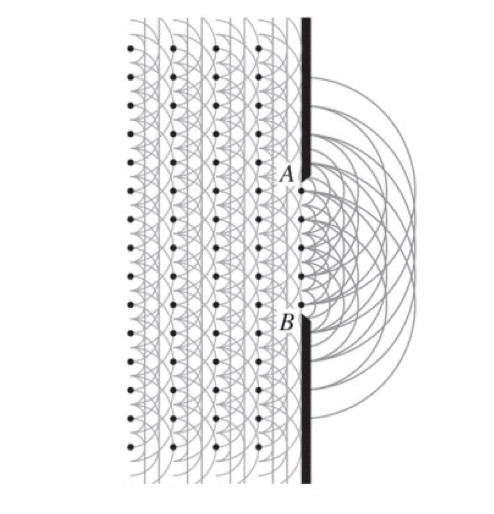
\includegraphics[scale=0.63]{gu_fr.png}}
		\caption{Иллюстрация принципа Гюйгенса-Френеля при дифракции на щели. Плоская волна при распространении
в каждой плоскости даёт набор точечных источников сферических волн. При попадании на препятствие волны
вторичные точечные источники дают интерферирующие волны, которые складываются в дифракционную картину.}
	\end{figure}

\subsection{Дифракция Френеля и распределение интенсивности волнового поля в центре за круглым отверстием}
Рассмотрим бесконечный транспарант, в котором сделано круглое отверстие радиусом $R$ На это
отверстие падает плоская волна с длиной $\lambda$ а за ним на расстоянии $z$ расположен экран, на котором
ведётся наблюдение результирующей картины. Нас будет интересовать расчёт интенсивности в точке $P$
лежащей на оси симметрии системы (см. рис. 2).


\begin{figure}[H]
		\center{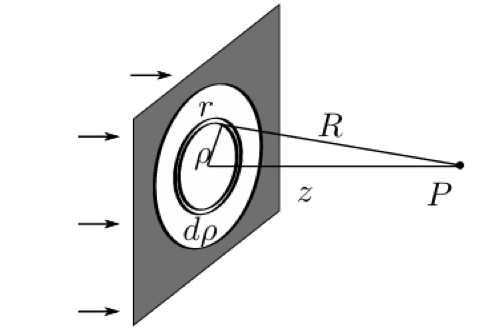
\includegraphics[scale=0.73]{raspr_intents.png}}
		\caption{Схема к постановке задачи о дифракции Френеля на круглом отверстии. Транспарант представляет собой
бесконечный поглощающий экран с круговым отверстием радиуса $R$ на оси симметрии системы на расстоянии $z$
находится точка $P$ наблюдения.}
	\end{figure}


Для применения принципа Гюйгенса-Френеля разобьем открытую часть волнового фронта (поверхность,
совпадающую с плоскостью отверстия) на узкие концентрические кольцевые зоны — \textit{зоны Френеля}.
Границы зон проводятся так, чтобы расстояние от края каждой зоны до точки $P$ отличалось ровно на $\lambda/2$
(т.е. расстояние от точки наблюдения $P$ до точек кольца \textit{$z + m\lambda/2$}, где $m$ – целое число). Это означает,
что вторичные волны от соседних зон приходят в точку в противофазе. Исходя из такого определения, мы
можем записать для $m$-ой зоны Френеля разность хода по отношению к центральному источнику:


\begin{equation}
\Delta_m = \sqrt{z^2 + r_m^2} - z \approx \frac{r_m^2}{2z} = \frac{m\lambda}{2},
\end{equation}

откуда радиус $m$-й зоны Френеля равен

\begin{equation}
r_m = \sqrt{m\lambda z}.
\end{equation}

Вклады соседних зон приходят в точку наблюдения практически в противофазе, поэтому суммирование амплитуд удобно представлять векторной диаграммой. Такая диаграмма приводит к спирали Френеля.

Характерное свойство спирали Френеля заключается в том, что, когда открыто нечетное число зон, конец
вектора оказывается в верхней части спирали (далеко от первого вектора), что даёт максимум
интенсивности. Когда открыто четное число зон — в нижней части (близко к первому вектору), что дает
минимум.

\begin{figure}[H]
		\center{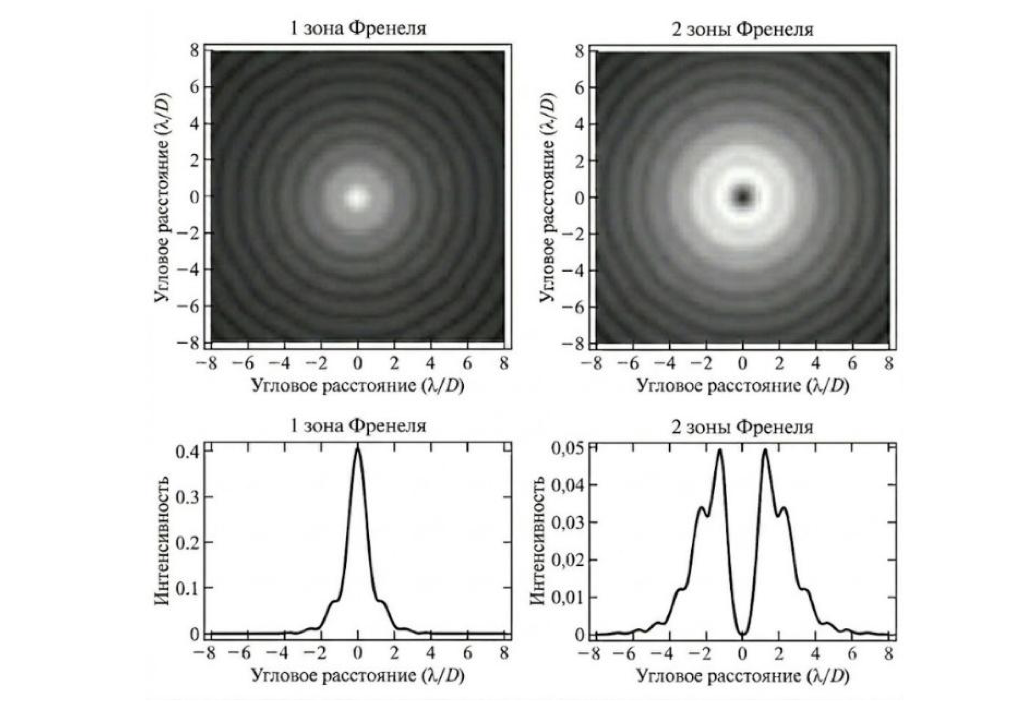
\includegraphics[scale=0.73]{hernya.png}}
		\caption{результат распределения интенсивности в плоскости наблюдения. Центр наблюдения отвечает точке $P$. $D$ –
диаметр открытого отверстия}
	\end{figure}

Удобно ввести число открытых зон Френеля
$N = \frac{r^2}{\lambda z}$ и волновой параметр $p = \frac{r}{\sqrt{\lambda z}} = \sqrt{N}.$

Тогда можно выделить три режима:
\begin{enumerate}[label=\arabic*)]
    \item предел геометрической оптики: $p \ll 1$;
    \item дифракция Френеля: $p \sim 1$;
    \item дифракция Фраунгофера: $p \gg 1$.
\end{enumerate}



\subsection{Дифракция на круглом отверстии}

При дифракции плоской волны на круглом отверстии в непрозрачном экране на удалённой плоскости
наблюдения (при условии $p \gg 1$) образуется картина дифракции, показанная на Рис.4 : центральное
яркое дифракционное пятно (которое называется пятном Эйри) окружено чередующимися светлыми и
тёмными кольцами. Угловая полуширина пятна Эйри (главного максимума в
картине $I(\theta)$ определяется условием

\begin{equation}
\sin\theta = 0.61\,\frac{\lambda}{r}.
\end{equation}

\begin{figure}[H]
		\center{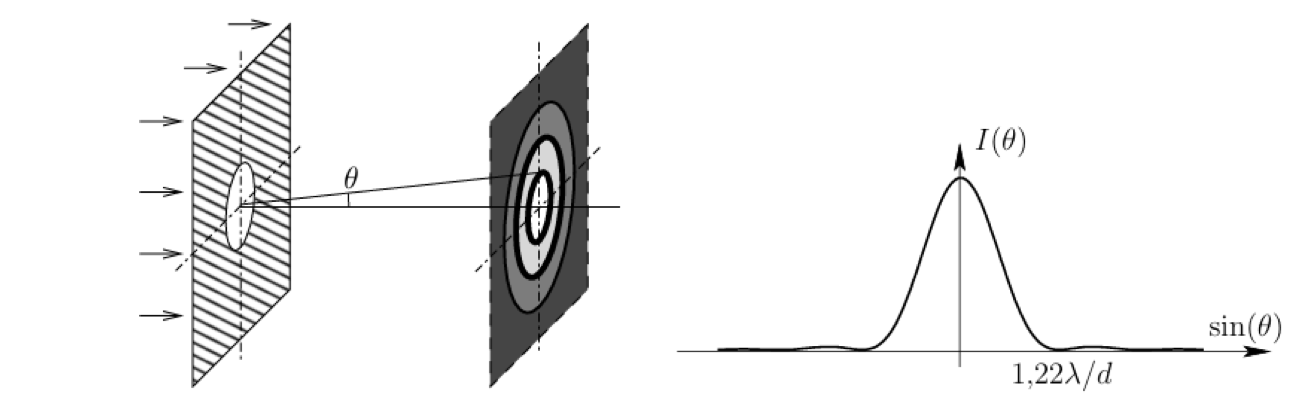
\includegraphics[scale=0.73]{another_bullshit.png}}
		\caption{Слева - геометрия задачи дифракции Фраунгофера на круглом отверстии. Справа - угловое распределение интенсивности в центральном сечении. Дифракционная картина сосредоточена в основном в главном дифракционном максимуме.}
	\end{figure}



% Для круглого непрозрачного препятствия используется принцип Бабине: сумма амплитуд полей, получаемых от двух взаимно дополнительных экранов, равна амплитуде поля при отсутствии экрана. Это позволяет свести задачу дифракции на непрозрачном диске к задаче дифракции на отверстии той же формы и, в частности, объяснить наличие пятна Пуассона в центре тени.




\subsection{Дифракция Френеля на щели}

Рассмотрим дифракцию плоской волны на щели, считая заданной её ширину $b$, а длину – бесконечной для
одномерности задачи. Пусть точка наблюдения $P$ расположена на расстоянии $z$ от щели.

\begin{figure}[H]
		\center{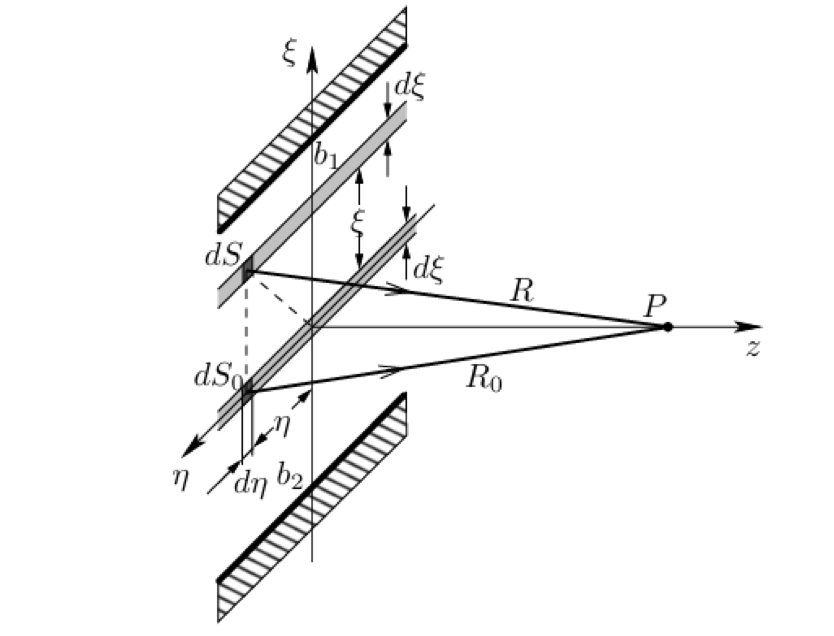
\includegraphics[scale=0.43]{more_bullshit.png}}
		\caption{Схема к постановке задачи о дифракции Френеля на щели. Транспарант представляет собой бесконечный поглощающий экран с горизонтальной щелью ширины $b$}
	\end{figure}


Разобьём щель на узкие полоски ширины $d\xi$, параллельные её краям. Разность фаз между соседними полосками равна

$$
d\varphi = k\left(\sqrt{z^2 + (\xi + d\xi)^2} - \sqrt{z^2 + \xi^2}\right)
\approx k\frac{\xi\,d\xi}{z},
$$

где $k = 2\pi/\lambda$. В данном случае вместо кольцевых зон Френеля, отвечающим колебаниям с набором фазы $\pi$
получаются зоны в виде полос (их называют \textit{зонами Шустера}) на расстояниях 
\begin{equation}
\xi_m = \sqrt{m\lambda z}.
\end{equation}
от точки наблюдения $P$.

В результате наблюдений дифракции Френеля на щели можно сопоставить распределение интенсивности
в соответствующей точке: 

\begin{figure}[H]
		\center{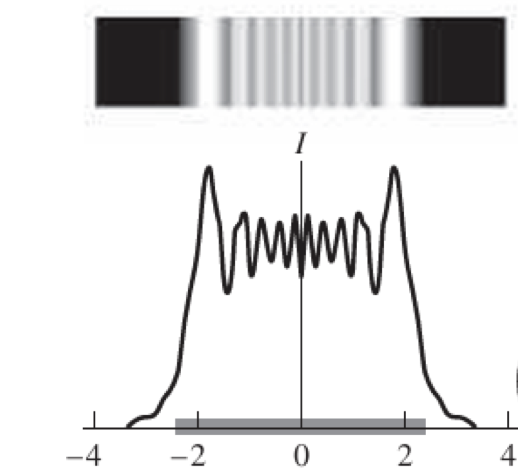
\includegraphics[scale=0.53]{greater_bullshit.png}}
		\caption{Сверху - пример дифракционной френелевской картины на щели. Снизу - распределение интенсивности по ширине щели}
	\end{figure}


\subsection{Дифракция Фраунгофера на щели}
Дифракция Фраунгофера (дифракция в дальней волновой зоне, или дифракция в параллельных лучах)
наблюдается в случае большого волнового параметра, что при заданных геометрических параметрах
препятствия она наблюдается на больших расстояниях. Оценим дальность для щели шириной $b$ = 1 мм и 
$\lambda$ = 500 нм: $z =
b^2/\lambda = 2 $ м. Для локализации этой картины используют дополнительную линзу за 
препятствием, фокусирующие параллельные лучи в соответствующие точки в фокальной плоскости.
На Рис.7 изображена типичная схема по наблюдению дифракции Фраунгофера на щели.

\begin{figure}[H]
		\center{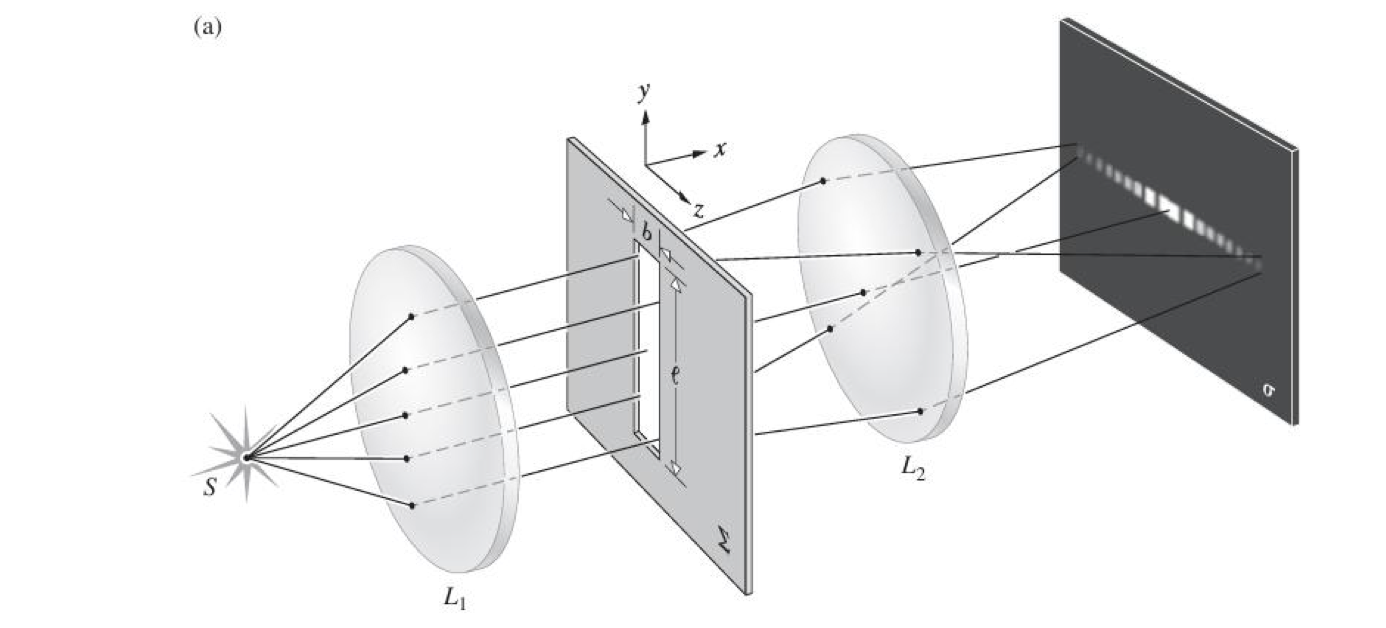
\includegraphics[scale=0.43]{very_bullshit.png}}
		\caption{Типичная схема для наблюдения дифракции Фраунгофера на щели. Тонкая линза $L_1$ преобразует волновой
фронт от источника $S$ в плоский для освещения щели, находящейся в плоскости транспаранта $\Sigma$. Прошедшее
излучение фокусируется линзой $L_2$ на экран.}
	\end{figure}

\begin{figure}[H]
		\center{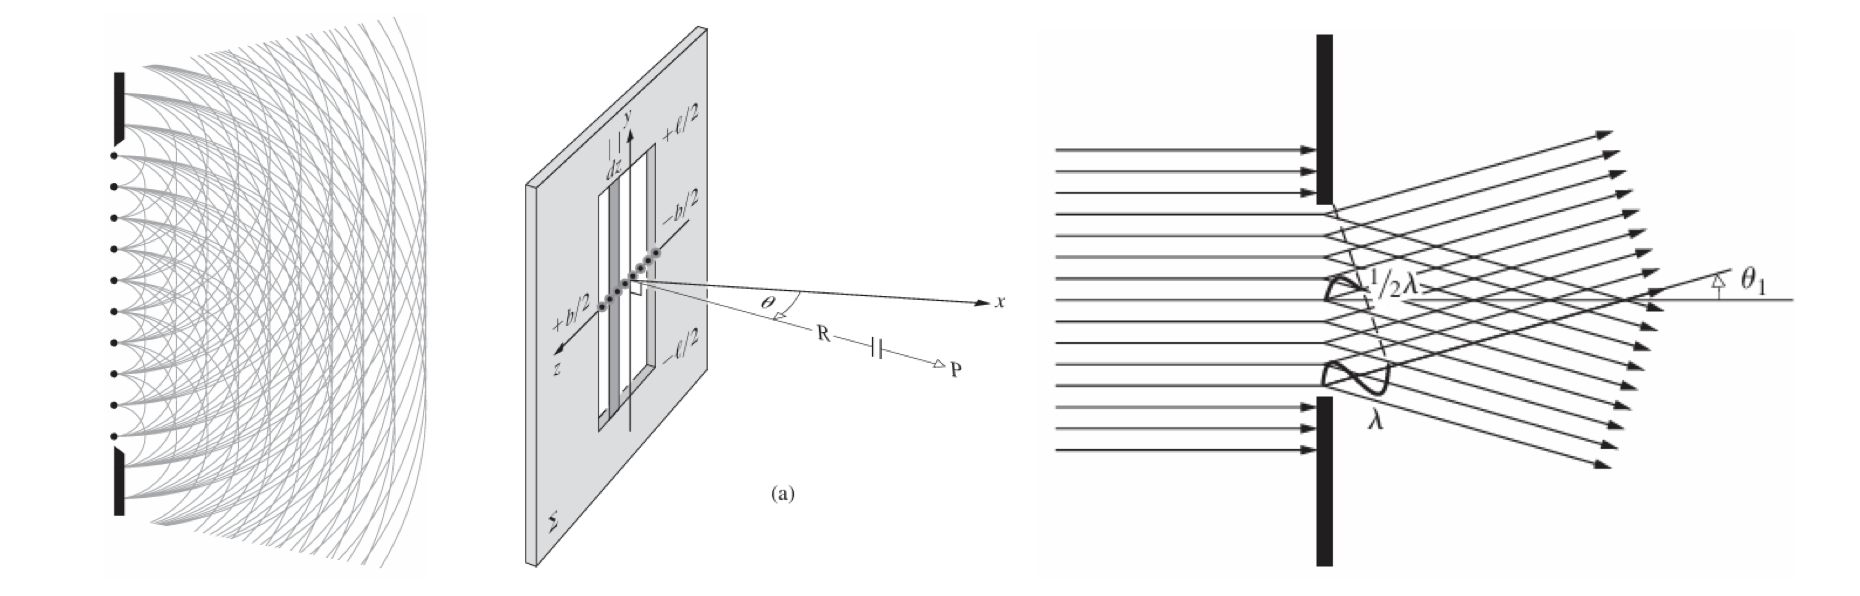
\includegraphics[scale=0.53]{badass_bullshit.png}}
		\caption{Представление волны в плоскости щели и за ней в виде суперпозиции волн от точечных источников}
	\end{figure}




Пусть щель разбита на $N$ одинаковых элементарных источников, находящихся на расстоянии $d$ друг от друга, так что $b = Nd$. Тогда разность фаз между соседними источниками равна

\begin{equation}
\alpha = kd\sin\theta.
\end{equation}

Суммарная амплитуда поля оказывается пропорциональной

\begin{equation}
E(\theta) \propto \frac{\sin(N\alpha/2)}{\sin(\alpha/2)}.
\end{equation}

В пределе $N \gg 1$ для интенсивности получаем классическую формулу дифракции Фраунгофера на щели:

\begin{equation}
I(\theta) = I(0)\left(\frac{\sin\beta}{\beta}\right)^2,
\qquad
\beta = \frac{\pi b\sin\theta}{\lambda}.
\end{equation}

Минимумы интенсивности(темные полосы) определяются условием

\begin{equation}
b\sin\theta_n = n\lambda,
\qquad n = \pm 1, \pm 2, \ldots
\end{equation}

а в фокальной плоскости линзы с фокусным расстоянием $f$ их координаты равны

\begin{equation}
x_n = f\tan\theta_n \approx \frac{fn\lambda}{b}.
\end{equation}


\subsection{Дифракция Фраунгофера на двух щелях}

Для двух одинаковых щелей ширины $b$, расстояние между которыми равно $d$, распределение интенсивности представляет собой интерференционные полосы, модулированные дифракционной огибающей:

\begin{equation}
I(\theta) = I(0)\left(\frac{\sin\beta}{\beta}\right)^2 \bigl(1 + \cos(kd\sin\theta)\bigr).
\end{equation}

Положения интерференционных максимумов определяются соотношением

\begin{equation}
d\sin\theta_m = m\lambda,
\qquad m = 0, \pm 1, \pm 2, \ldots
\end{equation}


а расстояние между соседними интерференционными полосами в фокальной плоскости линзы равно

\begin{equation}
\delta x = \frac{f\lambda}{d}.
\end{equation}


Поскольку полная угловая ширина главного дифракционного максимума (от минимума до минимума)
равна $2 \lambda / b$, где $b$ — ширина отдельной щели, то на нём укладывается $N = 2d/b$ тёмных
интерференционных полос (в центре картины максимум, поэтому светлых полос — на одну больше).

\begin{figure}[H]
		\center{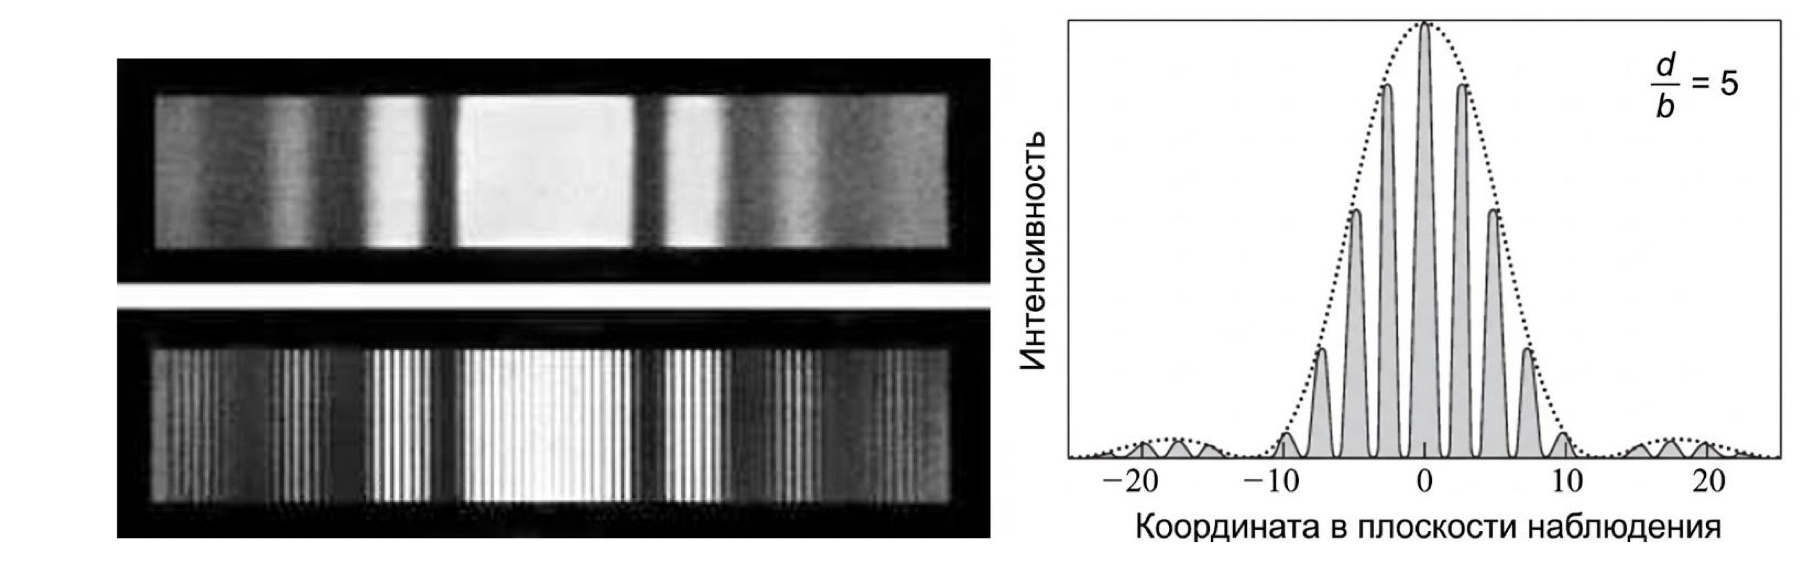
\includegraphics[scale=0.53]{comprehensive_bullshit .png}}
		\caption{Слева - картины дифракции на одной щели (сверху) и на двух одинаковых щелях той же ширины(снизу). Справа - распределение
интенсивности за двойной щелью.}
	\end{figure}




Для наблюдения чёткой интерференционной картины необходимо, чтобы расстояние между щелями не превышало радиус когерентности источника:

\begin{equation}
d \leq \rho_{\text{ког}} \approx \frac{\lambda f_1}{a},
\end{equation}

где $a$ --- размер протяжённого источника света, а $f_1$ --- фокусное расстояние линзы, формирующей плоскую волну.

\section{{Ход работы}}

\textbf{Цель работы:} исследовать явления дифракции Френеля на щели, протяжённом препятствии, круглом отверстии и круглом препятствии, а также дифракцию Фраунгофера на одной и двух щелях; проверить теоретические соотношения для положения максимумов при дифракции Френеля и Фраунгофера.

\subsection{Описание установки и работа с установкой}

Оборудование установки включает оптическую скамью, зрительную трубу, микроскоп с видеокамерой, набор рейтеров, оптические щели, кассету с круглыми отверстиями, собирающие линзы, двойную щель, линейное и круглые препятствия, калибровочный слайд, юстировочный экран, источник света и персональный компьютер для регистрации дифракционных картин.

\subsection{Внешний вид компонент экспериментальной установки}

\imgplaceholder{Оптическая скамья.}{Рис.~1a. Оптическая скамья.}
\imgplaceholder{Зрительная труба.}{Рис.~2a. Зрительная труба.}
\imgplaceholder{Микроскоп.}{Рис.~3a. Микроскоп.}
\imgplaceholder{Рейтер трёхкоординатный.}{Рис.~4a. Рейтер трёхкоординатный.}
\imgplaceholder{Рейтер на широкой каретке.}{Рис.~5a. Рейтер на широкой каретке.}
\imgplaceholder{Рейтер на узкой каретке.}{Рис.~6a. Рейтер на узкой каретке.}
\imgplaceholder{Оптическая щель с микрометрическим винтом.}{Рис.~7a. Оптическая щель с микрометрическим винтом.}
\imgplaceholder{Кассета с круглыми диафрагмами.}{Рис.~8a. Кассета с круглыми диафрагмами.}
\imgplaceholder{Собирающая линза в оправе.}{Рис.~9a. Собирающая линза в оправе.}
\imgplaceholder{Двойная щель.}{Рис.~10a. Двойная щель.}
\imgplaceholder{Линейное препятствие.}{Рис.~11a. Линейное препятствие.}
\imgplaceholder{Система круглых препятствий.}{Рис.~12a. Система круглых препятствий.}
\imgplaceholder{Калибровочный слайд.}{Рис.~13a. Калибровочный слайд.}
\imgplaceholder{Юстировочный экран.}{Рис.~14a. Юстировочный экран.}
\imgplaceholder{Источник света.}{Рис.~15a. Источник света.}
\imgplaceholder{Источник света, вид из дополнения к установке.}{Рис.~I. Источник света.}

\subsection{Ход работы}

Перед началом измерений необходимо:
\begin{enumerate}
    \item выставить и зафиксировать источник света на оптической скамье;
    \item определить высоту оптической оси с помощью кассеты с круглыми диафрагмами;
    \item отъюстировать экран и щель так, чтобы прошедший свет попадал в центр юстировочного экрана;
    \item установить собирающую линзу и добиться фокусировки пучка вблизи центра экрана;
    \item настроить зрительную трубу на бесконечность и убедиться, что плоскость щели находится в фокальной плоскости линзы;
    \item установить микроскоп и провести его калибровку по калибровочному слайду.
\end{enumerate}

\paragraph{Калибровка микроскопа.}
В программе наблюдения необходимо получить резкое изображение калибровочной шкалы, измерить её длину в пикселях и определить коэффициент пересчёта пикселей в реальные размеры. Все дальнейшие измерения дифракционных картин выполняются в пикселях с последующим пересчётом в миллиметры или микрометры.

\subsection{I. Дифракция Френеля}

Для наблюдения дифракции Френеля собирают схему: источник света, первая щель как вторичный источник, линза, исследуемая щель или препятствие и микроскоп. После получения резкого изображения щели микроскоп постепенно смещают вдоль оптической оси и наблюдают возникновение тёмных дифракционных полос.

\imgplaceholder{Схема установки для наблюдения дифракции Френеля.}{Рис.~1. Схема установки для наблюдения дифракции Френеля.}

В ходе измерений:
\begin{enumerate}
    \item фиксируют начальное положение микроскопа, соответствующее резкому изображению щели;
    \item измеряют смещение $z$ для различных чисел наблюдаемых тёмных полос;
    \item определяют ширину щели двумя способами: по микрометрическому винту и по изображению на мониторе;
    \item повторяют измерения для другой ширины щели;
    \item исследуют дифракцию Френеля на линейном препятствии и проверяют наличие светлого центра при чётном числе тёмных полос.
\end{enumerate}

При обработке результатов строят зависимость расстояния $z$ от числа открытых зон Френеля и сравнивают экспериментальные данные с теоретическими соотношениями.

\end{document}
